\documentclass[a4paper, 11pt]{article}
\usepackage[spanish]{babel}
\selectlanguage{spanish}
\usepackage{graphicx}
\usepackage{wrapfig}
\usepackage[utf8]{inputenc}
\usepackage{amsmath}
\usepackage{dsfont}
\usepackage{multirow}
\usepackage{vmargin}
\usepackage{subfigure}
\usepackage[numbers, sort&compress]{natbib}
\usepackage{url}
\usepackage{cite}
\usepackage{wrapfig}
\usepackage{enumerate} 
\usepackage{sectsty} % centrar secciones de encabezados
\usepackage[usenames]{color}
\usepackage{caption}
\usepackage{amsfonts}
\usepackage{amssymb}
\usepackage{listings}
\usepackage{color}
\usepackage{algpseudocode}
\usepackage{multirow}
\usepackage[usenames]{color}
\usepackage{epstopdf}
\usepackage{float}
\usepackage{nameref}

\setmargins
{2.5cm}                        % margen izquierdo
{1cm}                         % margen superior
{16.5cm}                      % anchura del texto
{23.42cm}                    % altura del texto
{10pt}                           % altura de los encabezados
{0cm}                           % espacio entre el texto y los encabezados
{0pt}                             % altura del pie de página
{1cm}                           % espacio entre el texto y el pie de página

\definecolor{mygreen}{rgb}{0,0.6,0}
\definecolor{mygray}{rgb}{0.5,0.5,0.5}
\definecolor{mymauve}{rgb}{0.58,0,0.82}

\lstset{ 
  backgroundcolor=\color{white},   % choose the background color; you must add \usepackage{color} or \usepackage{xcolor}; should come as last argument
  basicstyle=\footnotesize,        % the size of the fonts that are used for the code
  breakatwhitespace=false,         % sets if automatic breaks should only happen at whitespace
  breaklines=true,                 % sets automatic line breaking
  captionpos=b,                    % sets the caption-position to bottom
  commentstyle=\color{mygreen},    % comment style
  deletekeywords={...},            % if you want to delete keywords from the given language
  escapeinside={\%*}{*)},          % if you want to add LaTeX within your code
  extendedchars=true,              % lets you use non-ASCII characters; for 8-bits encodings only, does not work with UTF-8
  firstnumber=1,                % start line enumeration with line 1000
  frame=single,	                   % adds a frame around the code
  keepspaces=true,                 % keeps spaces in text, useful for keeping indentation of code (possibly needs columns=flexible)
  keywordstyle=\color{blue},       % keyword style
  language=Octave,                 % the language of the code
  morekeywords={*,...},            % if you want to add more keywords to the set
  numbers=left,                    % where to put the line-numbers; possible values are (none, left, right)
  numbersep=5pt,                   % how far the line-numbers are from the code
  numberstyle=\tiny\color{mygray}, % the style that is used for the line-numbers
  rulecolor=\color{black},         % if not set, the frame-color may be changed on line-breaks within not-black text (e.g. comments (green here))
  showspaces=false,                % show spaces everywhere adding particular underscores; it overrides 'showstringspaces'
  showstringspaces=false,          % underline spaces within strings only
  showtabs=false,                  % show tabs within strings adding particular underscores
  stepnumber=1,                    % the step between two line-numbers. If it's 1, each line will be numbered
  stringstyle=\color{mymauve},     % string literal style
  tabsize=2,	                   % sets default tabsize to 2 spaces
  title=\lstname                   % show the filename of files included with \lstinputlisting; also try caption instead of title
}


\begin{document}

\title{Representación de redes a través de la teoría de grafos}
\author{Serna Mendoza Jorge Armando\\
\small{Optimización de flujo en redes}}
\date{ }
\maketitle

\vspace{-1 cm}
\begin{center}\rule{\textwidth}{0.1mm} \end{center}
\vspace{-1.3 cm}
\begin {center}
\item \Large{\textbf{ Resumen}}
\end {center}

Este trabajo busca representar redes mediante la teoría de grafos, con la implementación de la librería \color{blue}NetworkX\color{black} \  de \texttt{Python}. A cada tipo de grafo se le identifica una aplicacion práctica y  se representa con un ejemplo inspirado en datos reales.
\vspace{-0.5cm}
\begin{center}\rule{\textwidth}{0.1mm} \end{center}


\section*{\centering{Introducción}}
Un \textit{grafo} $G=(N, A)$ es una pareja ordenada en la que $N$ es un conjunto de \textit{nodos} y $A$ es un conjunto de \textit{arcos}. El conjunto $A$ se conforma de pares de nodos $(u, v)$ y se dice que $u$ y $v \ \epsilon \ N$ son adyacentes. En $G$ se representa la adyacencia de $u$ con $v$, mediante una línea que une el nodo $u$ con el nodo $v$.
\\ \\
Un \textit{multigrafo} es un grafo que tiene \textit{multiarcos}, es decir,  si $u$ y $v$ son adyacentes, existe mas un arco que une a $u$ con $v$. Por otro lado, un \textit{ciclo} es una sucesión de nodos y arcos tales que forman un camino que comienza y termina en el mismo nodo. 

\section*{Grafo simple no dirigido acíclico}

Es un grafo $G = (N, A)$ que cumple:
\begin{itemize}
\item $G$ no tiene multiarcos.
\item Los arcos $(u, v) \ \epsilon \ A$ no tienen dirección $\forall \ u, v \ \epsilon \ N$.
\item $G$ no tiene ciclos.
\end{itemize}

\textbf{Ejemplo:} La Filogenia es la relación de parentesco entre especies, se encarga de estudiar filiación de entidades que derivan unas de otras en un proceso evolutivo. Véase figura (\ref{imagen1}).


\begin{table}[H]
\begin{center}
\caption{Bacterias.}
\begin{tabular}{|l|l|}
\hline 
 Notación  &Nombre \\  \hline \hline
a &Aquifex  \\ \hline
b &Thermotoga\\ \hline
c  &Planctomyces \\ \hline
d  &Cianobacteria\\ \hline
e  &Proteobacteria \\ \hline
f  &Spirochaetes\\ \hline
g  & Cytophaga\\ \hline
h  & Gram positiva\\ \hline
\end{tabular}
\label{tabla1}
\end{center}
\end{table}

\begin{figure}[H]
  \centering
    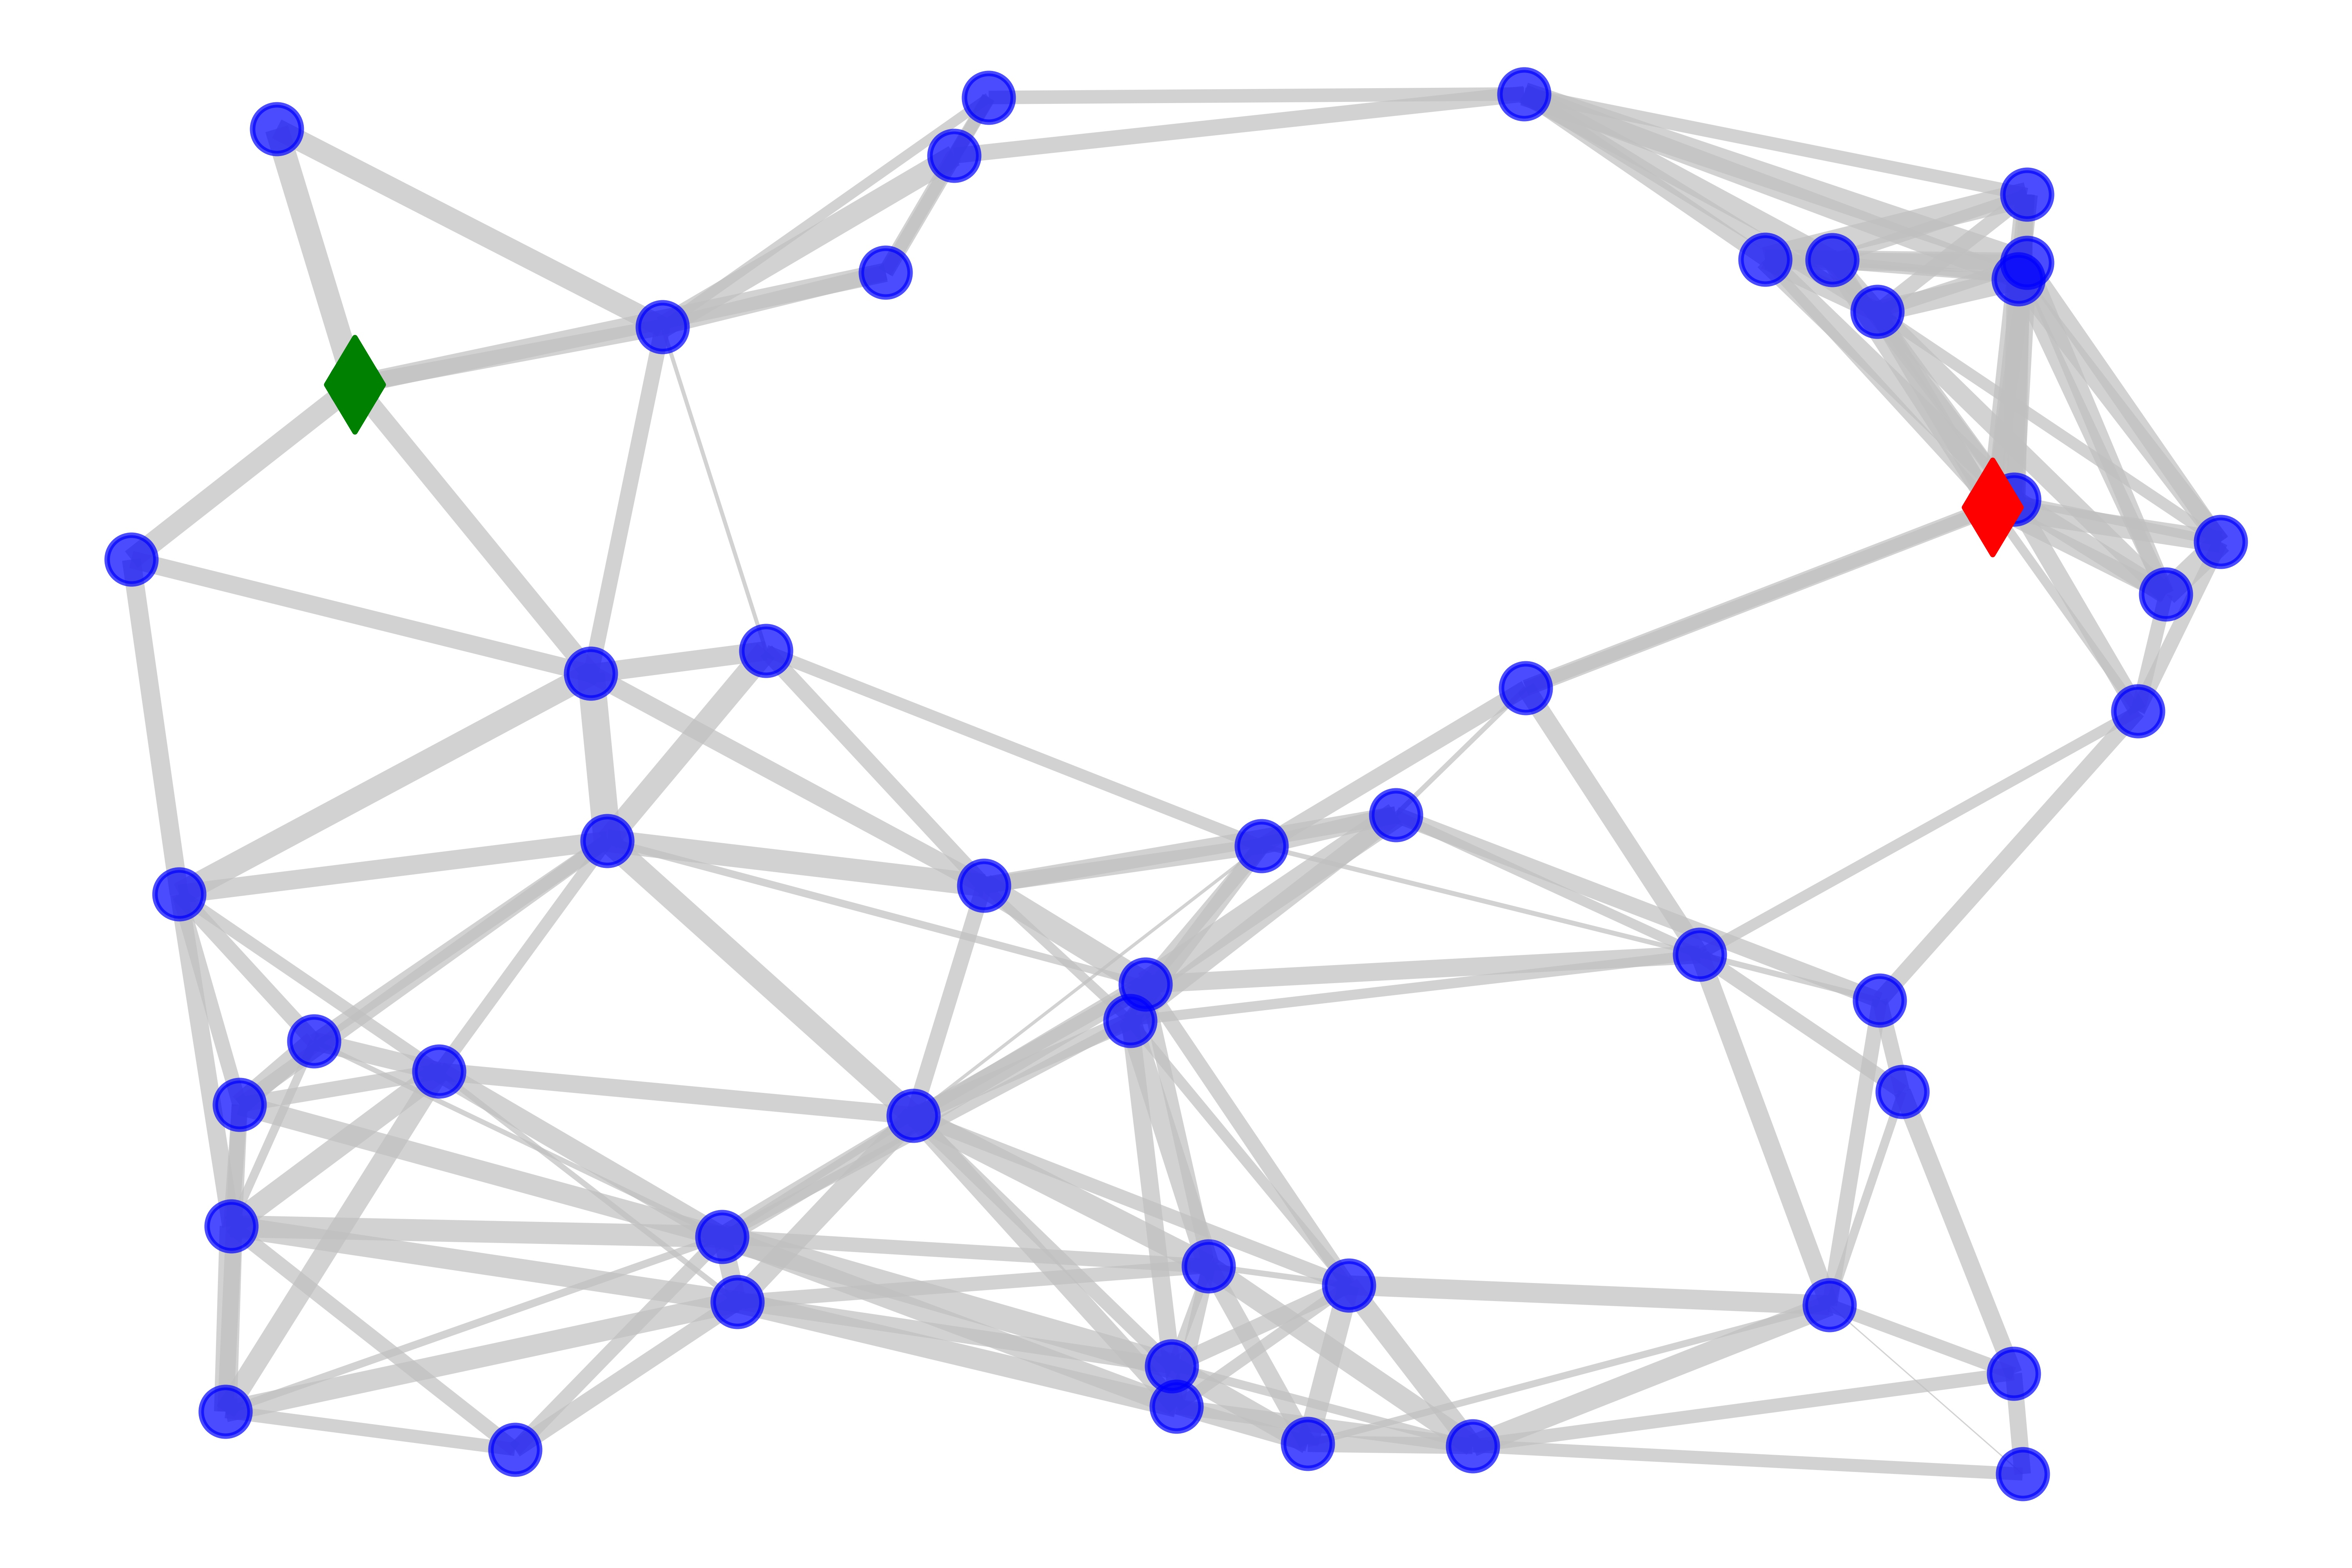
\includegraphics[scale=0.6]{grafo1}
  \caption{Árbol filogenético de la Bacteria}
  \label{imagen1}
\end{figure}

\textbf{Código en Python de la figura (\ref{imagen1}).}
\begin{lstlisting}[language=Python]
import networkx as nx
import matplotlib.pyplot as plt

#1 grafo simple no dirigido
G=nx.Graph()
G.add_edges_from([("Bacteria","a"), ("Bacteria","b"),("Bacteria","c"),("Bacteria","d"),("Bacteria","e"),("Bacteria","f"),("Bacteria","g"),("Bacteria","h")])
node1 = {"Bacteria"}
node2 = {"a", "b", "c","d","e", "f", "g", "h"}
pos = {"Bacteria":(0, 0),"a":(0,5), "b":(-5,5), "c":(-5,0), "d":(-5,-5), "e":(0,-5), "f":(5,-5), "g":(5,0), "h":(5,5)}
nx.draw_networkx_nodes(G, pos, nodelist=node1,node_size=5000, 
                       node_color='green', node_shape='o', width=5, alpha=1)
nx.draw_networkx_nodes(G, pos, nodelist=node2,node_size=400, 
                       node_color='green', node_shape='o', width=5, alpha=1)
nx.draw_networkx_edges(G, pos, width=3, alpha=0.5, edge_color='grey')
nx.draw_networkx_labels(G, pos, font_size=18)
plt.axis('off')
plt.savefig('grafo1.eps', format='eps', dpi=1000)
\end{lstlisting}

%%%%%%%%%%%%%%%%%%%%%%%%%
%%%%%%%%%%%%%%%%%%%%%%%%%
%%%%%%%%%%%%%%%%%%%%%%%%%


\section*{Grafo simple no dirigido cíclico}

Es un grafo $G = (N, A)$ que cumple:
\begin{itemize}
\item $G$ no tiene multiarcos.
\item Los arcos $(u, v) \ \epsilon \ A$ no tienen dirección $\forall \ u, v \ \epsilon \ N$.
\item $G$ tiene por lo menos un ciclo.
\end{itemize}


\textbf{Ejemplo:} Travelling Salesman Problem (TSP) es un problema que consiste en dada una lista de ciudades ($n$) y las distancias entre cada par de ellas (aristas), determinar cual es la ruta más corta posible que visita cada ciudad una vez y al finalizar regresa a la ciudad origen. Véase figura (\ref{imagen2}).

\begin{figure}[H]
  \centering
    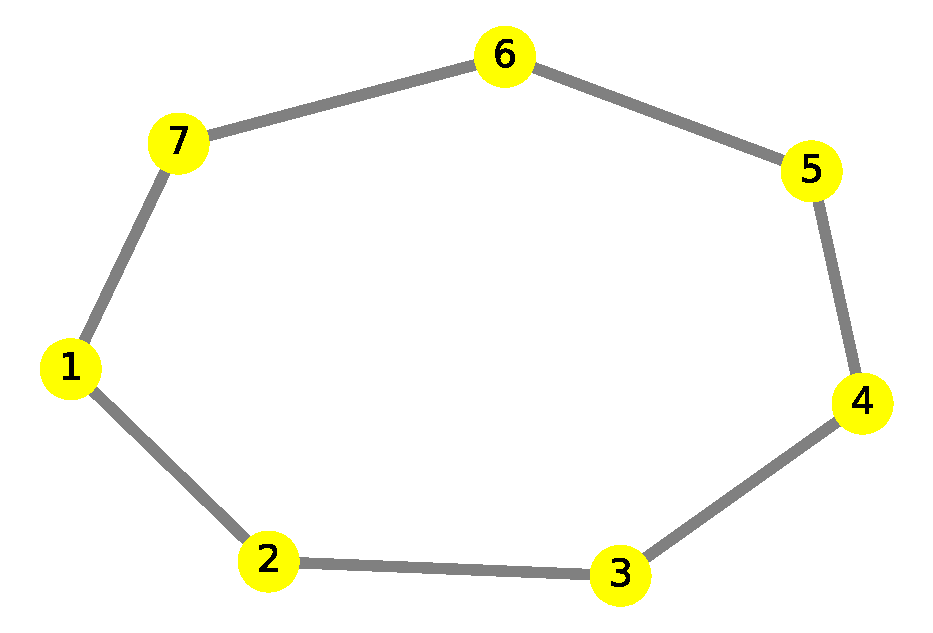
\includegraphics[scale=0.5]{grafo2}
  \caption{TSP con $n$=7}
  \label{imagen2}
\end{figure}


%%%%%%%%%%%%%%%%%%%%%%%%%
%%%%%%%%%%%%%%%%%%%%%%%%%
%%%%%%%%%%%%%%%%%%%%%%%%%


\section*{Grafo simple no dirigido reflexivo}

Es un grafo $G = (N, A)$ que cumple:
\begin{itemize}
\item $G$ no tiene multiarcos.
\item Los arcos $(u, v) \ \epsilon \ A$ no tienen dirección $\forall \ u, v \ \epsilon \ N$.
\item $G$ tiene por lo menos un nodo $u$ tal que la relacion $(u, u) \ \epsilon \ A$.
\end{itemize}


\textbf{Ejemplo:} (Producto Cartesiano). Sea $A = \{1, 2, 3, 4, 5, 6 \}$ un conjunto con 6 elementos y sea $A_{1} = \{1, 2, 3, 4, 5 \}$ un subconjunto de $A$. Se define el producto cartesiano $B = A \times A_{1}$.

 \[
   B = 
 \left \{ {\begin{array}{cccccc}
   (1,1) & (2,1) & (3,1) & (4,1) & (5,1) & (6,1) \\
   (1,2) &(2,2) &(3,2) &(4,2) &(5,2) &(6,2) \\
   (1,3) &(2,3) &(3,3) &(4,3) &(5,3) &(6,3) \\
   (1,4) &(2,4) &(3,4) &(4,4) &(5,4) &(6,4) \\  
   (1,5) &(2,5) &(3,5) &(4,5) &(5,5) &(6,5) \\
  \end{array} } \right \}
\] 

\begin{figure}[H]
  \centering
    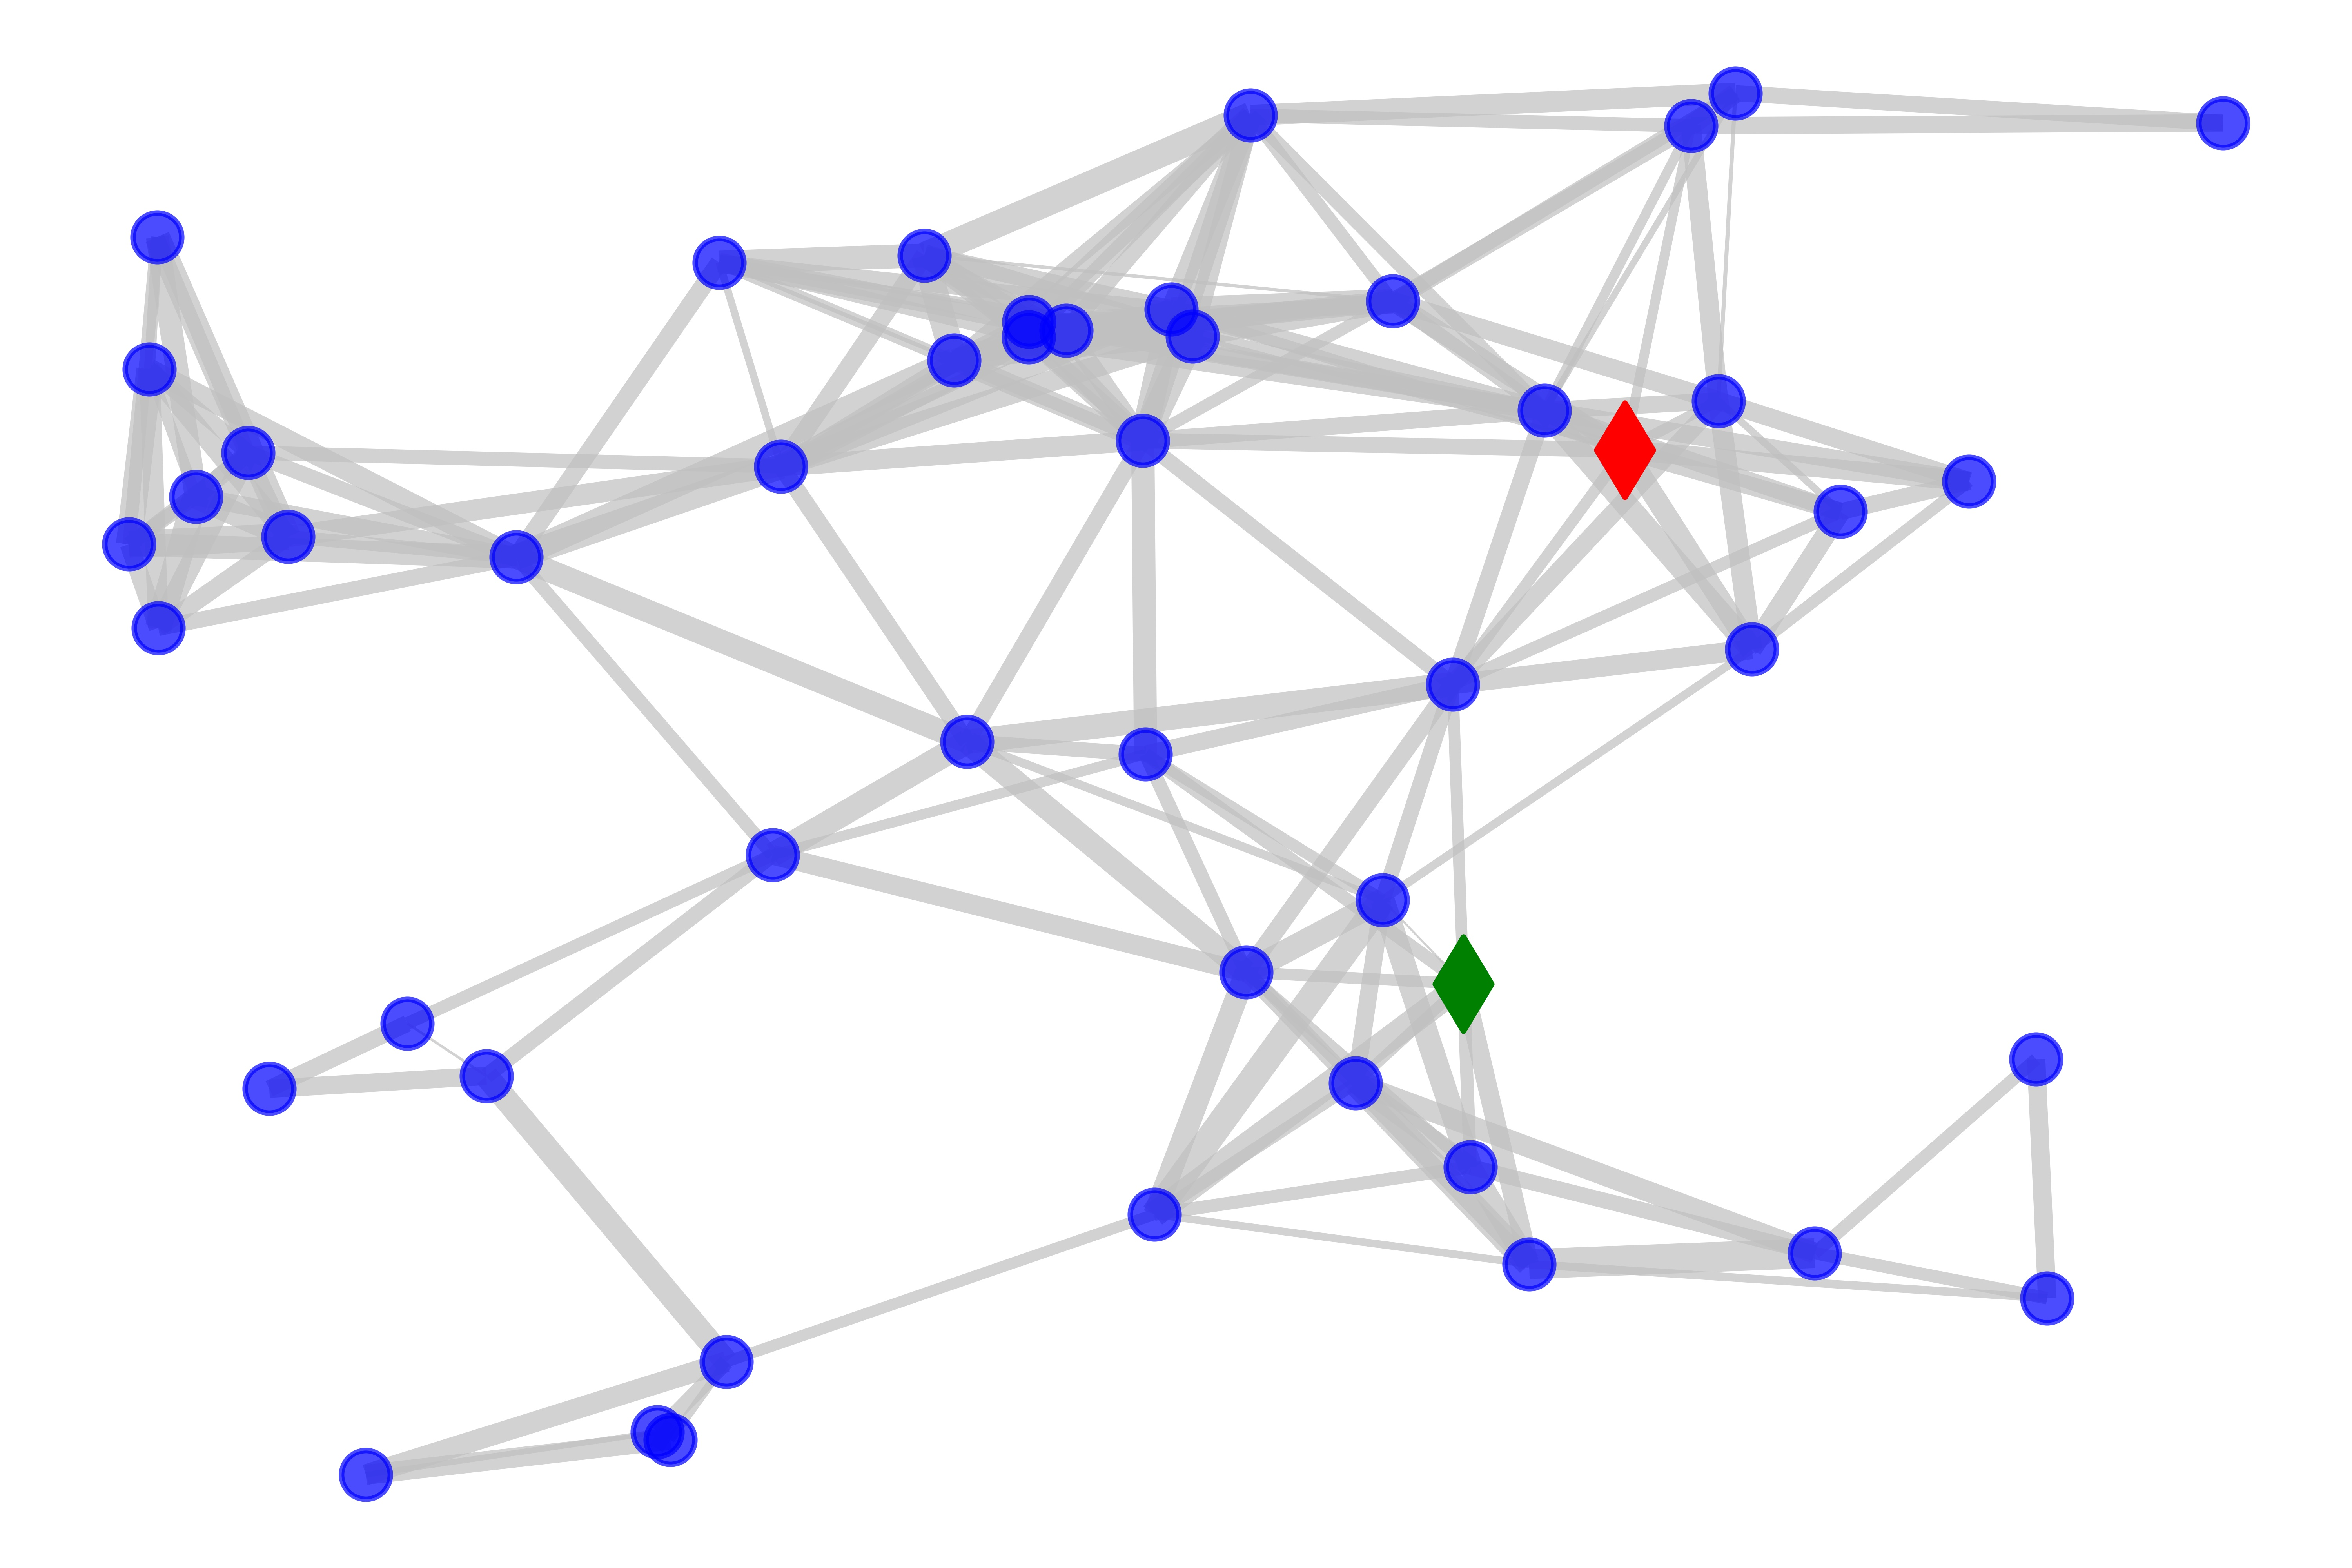
\includegraphics[scale=0.6]{grafo3}
  \caption{Representación de $B$ como un grafo}
  \label{imagen3}
\end{figure}

En la figura \ref{imagen3} se representa de color rojo a los nodos de $G$ que cumplen tener en $A$ arcos de la forma $(u, u)$.



%%%%%%%%%%%%%%%%%%%%%%%%%
%%%%%%%%%%%%%%%%%%%%%%%%%
%%%%%%%%%%%%%%%%%%%%%%%%%


\section*{Grafo simple dirigido acíclico }

Es un grafo $G = (N, A)$ que cumple:
\begin{itemize}
\item $G$ no tiene multiarcos.
\item Existe al menos un arco $(u, v) \ \epsilon \ A$ con dirección.
\item $G$ no tiene ciclos.
\end{itemize}


\textbf{Ejemplo:} (Árbol genealógico). Un árbol genealógico visto como un grafo, es una representación de los descendientes de un individuo de forma organizada. Véase figura (\ref{imagen4}).

\begin{figure}[H]
  \centering
    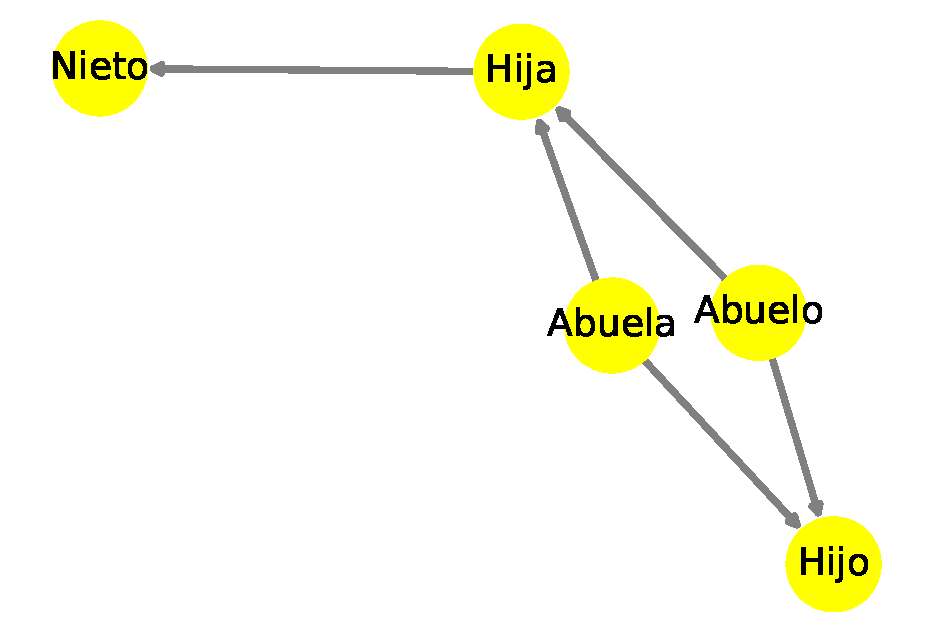
\includegraphics[scale=0.6]{grafo4}
  \caption{Ejemplo de un árbol genealógico}
  \label{imagen4}
\end{figure}



%%%%%%%%%%%%%%%%%%%%%%%%%
%%%%%%%%%%%%%%%%%%%%%%%%%
%%%%%%%%%%%%%%%%%%%%%%%%%


\section*{Grafo simple dirigido cíclico}

Es un grafo $G = (N, A)$ que cumple:
\begin{itemize}
\item $G$ no tiene multiarcos.
\item Existe al menos un arco $(u, v) \ \epsilon \ A$ con dirección.
\item $G$ tiene a lo menos un ciclo.
\end{itemize}


\textbf{Ejemplo:} (Ciclo Hidrológico). El ciclo hidrológico es el proceso de circulación del agua entre los distintos compartimentos que forman la hidrosfera, donde intervienen reacciones químicas que provocan cambios de estado físico del agua. Véase figura (\ref{imagen5}).

\begin{figure}[H]
  \centering
    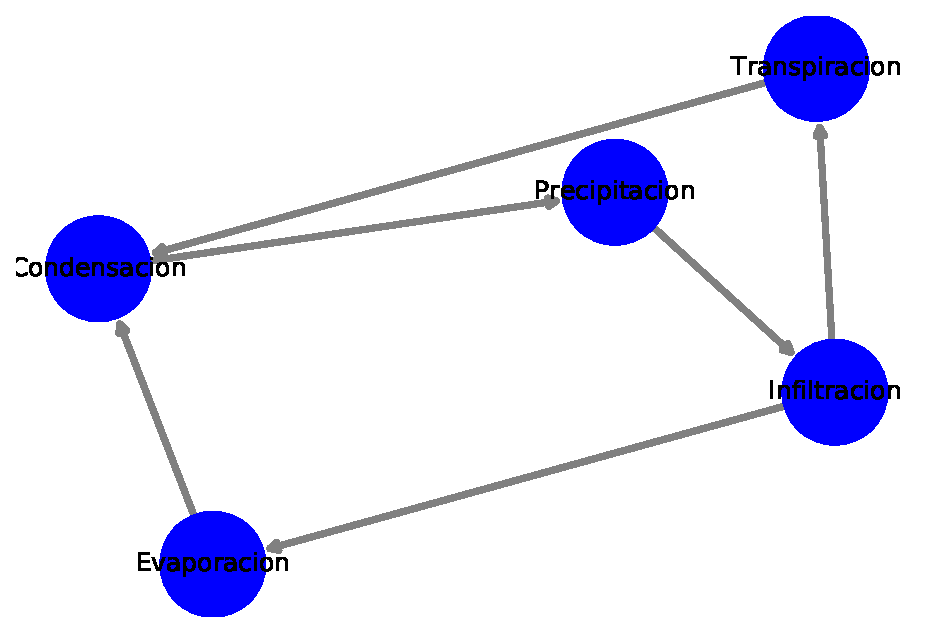
\includegraphics[scale=0.65]{grafo5}
  \caption{Ejemplo de un árbol genealógico}
  \label{imagen5}
\end{figure}




%%%%%%%%%%%%%%%%%%%%%%%%%
%%%%%%%%%%%%%%%%%%%%%%%%%
%%%%%%%%%%%%%%%%%%%%%%%%%


\section*{Grafo simple dirigido reflexivo}

Es un grafo $G = (N, A)$ que cumple:
\begin{itemize}
\item $G$ no tiene multiarcos.
\item Existe al menos un arco $(u, v) \ \epsilon \ A$ con dirección.
\item $G$ tiene por lo menos un nodo $u$ tal que la relacion $(u, u) \ \epsilon \ A$.
\end{itemize}


\textbf{Ejemplo:} (Estado del clima). Es la condición en que se encuentra la atmósfera en un determinado momento y lugar. Los estados del clima cambian todos los días con cierta probabilidad. Cuando se representa el clima mediante un grafo, los nodos representan los estados del clima y las aristas la probabilidad de pasar de un estado al otro. Véase figura (\ref{imagen6}).


\begin{table}[H]
\begin{center}
\caption{Estado del clima.}
\begin{tabular}{|l|l|}
\hline 
 Notación  &Clima \\  \hline \hline
1 &Lluvioso  \\ \hline
2 &Soleado\\ \hline
3  &Nublado \\ \hline
4  &Nevado\\ \hline
5  &Frío \\ \hline
6  &Ventoso\\ \hline
\end{tabular}
\label{tabla2}
\end{center}
\end{table}


\begin{figure}[H]
  \centering
    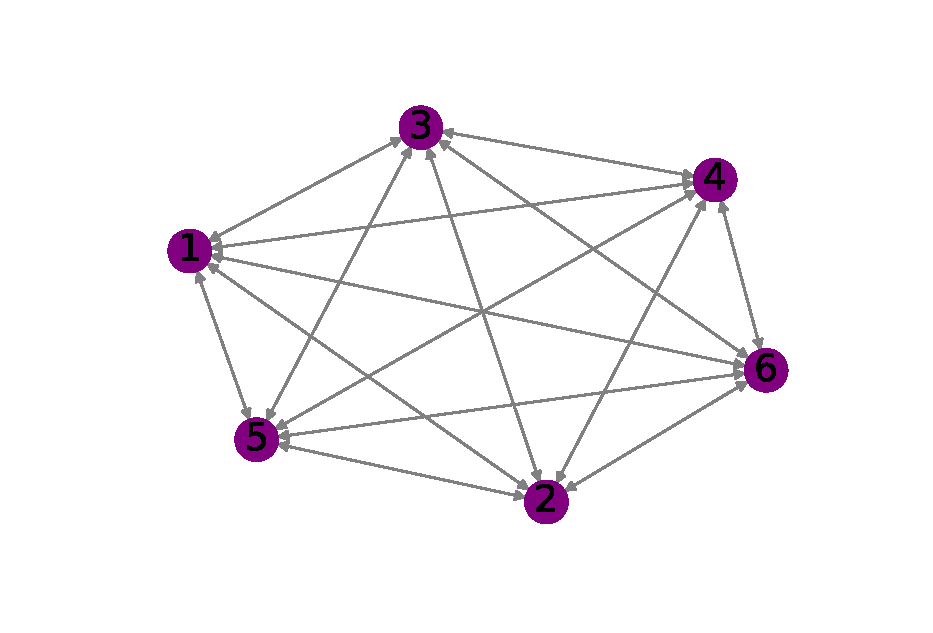
\includegraphics[scale=0.7]{grafo6}
  \caption{Estados del clima}
  \label{imagen6}
\end{figure}




%%%%%%%%%%%%%%%%%%%%%%%%%
%%%%%%%%%%%%%%%%%%%%%%%%%
%%%%%%%%%%%%%%%%%%%%%%%%%


\section*{Multigrafo no dirigido acíclico }

Es un grafo $G = (N, A)$ que cumple:
\begin{itemize}
\item $G$ tiene al menos un par de nodos, tales que tienen mas de una arista de adyacencia.
\item Los arcos $(u, v) \ \epsilon \ A$ no tienen dirección $\forall \ u, v \ \epsilon \ N$.
\item $G$ no tiene ciclos.
\end{itemize}


\textbf{Ejemplo:} (Red de rutas). Cuando una red de rutas se representa mediante un grafo, los nodos representan lugares y los arcos representan el camino que une esos lugares. En la figura (\ref{imagen7}) se considera las rutas de 4 ciudades, tales ciudades pueden tener un único camino (azul) para llegar de ciudad a ciudad o más de un camino (verde) para llegar de ciudad a ciudad.


\begin{figure}[H]
  \centering
    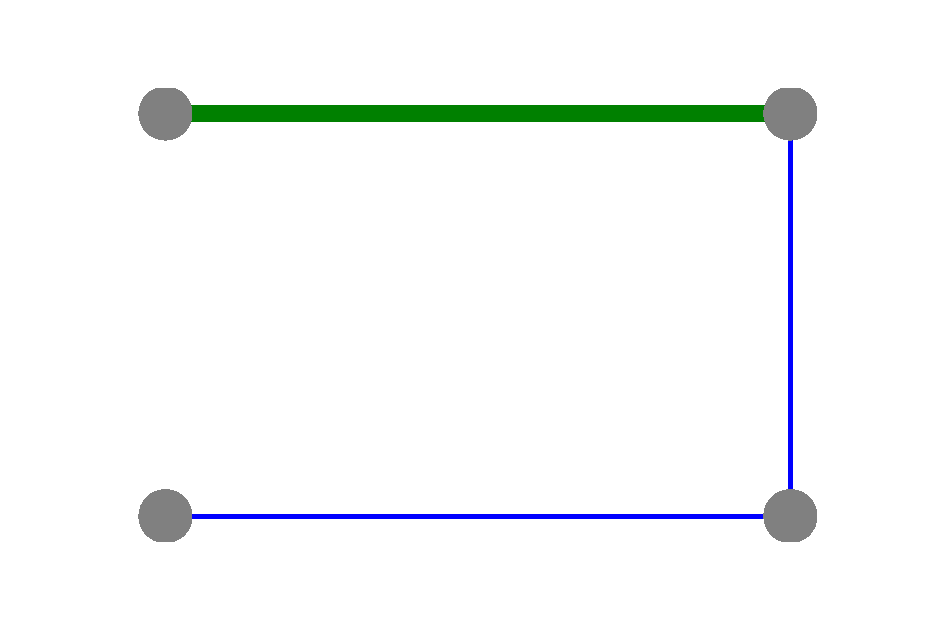
\includegraphics[scale=0.7]{grafo7}
  \caption{Red de rutas}
  \label{imagen7}
\end{figure}



%%%%%%%%%%%%%%%%%%%%%%%%%
%%%%%%%%%%%%%%%%%%%%%%%%%
%%%%%%%%%%%%%%%%%%%%%%%%%

\section*{Multigrafo no dirigido cíclico }


Es un grafo $G = (N, A)$ que cumple:
\begin{itemize}
\item $G$ tiene al menos un par de nodos, tales que tienen mas de una arista de adyacencia.
\item Los arcos $(u, v) \ \epsilon \ A$ no tienen dirección $\forall \ u, v \ \epsilon \ N$.
\item $G$ tiene a lo menos un ciclo.
\end{itemize}


\textbf{Ejemplo:} (Puentes de Königsberg). El problema consistía en encontrar un recorrido para cruzar a pie toda la ciudad, pasando sólo una vez por cada uno de los puentes, y regresando al mismo punto de inicio.  En la figura (\ref{imagen8}) se considera los 4 puntos de inicio posibles, tales puntos pueden tener un puente (azul) para llegar de un punto a otro punto o más de un puente (verde) para llegar de un punto a otro punto.


\begin{figure}[H]
  \centering
    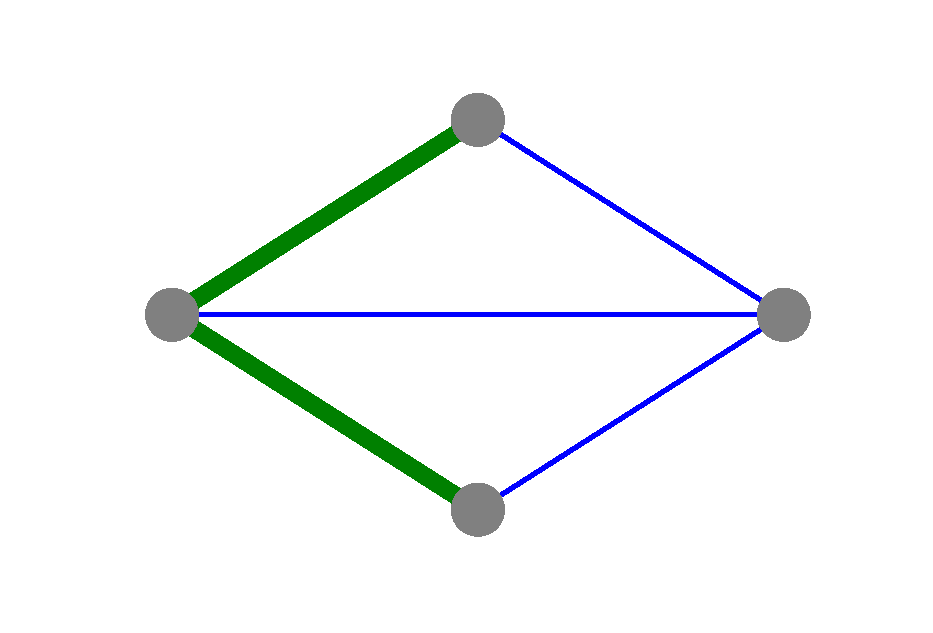
\includegraphics[scale=0.7]{grafo8}
  \caption{Puentes de Königsberg}
  \label{imagen8}
\end{figure}



%%%%%%%%%%%%%%%%%%%%%%%%%
%%%%%%%%%%%%%%%%%%%%%%%%%
%%%%%%%%%%%%%%%%%%%%%%%%%

\section*{Multigrafo no dirigido reflexivo }


Es un grafo $G = (N, A)$ que cumple:
\begin{itemize}
\item $G$ tiene al menos un par de nodos, tales que tienen mas de una arista de adyacencia.
\item Los arcos $(u, v) \ \epsilon \ A$ no tienen dirección $\forall \ u, v \ \epsilon \ N$.
\item $G$ tiene por lo menos un nodo $u$ tal que la relacion $(u, u) \ \epsilon \ A$.
\end{itemize}


\textbf{Ejemplo:} (Proceso de calidad). En la industria se aplican procesos de calidad a los productos antes de ser sacados al mercado. Cuando un proceso de calidad se representa mediante un grafo, el grafo tiene un nodo origen que representa el inicio del proceso, nodos intermedios que llevan a cabo cada tarea de revisión de calidad, la misma revisión se puede llevar a cabo más de una vez antes de ser pasado a otro proceso de calidad y un nodo destino que representa el gin del proceso.


\begin{figure}[H]
  \centering
    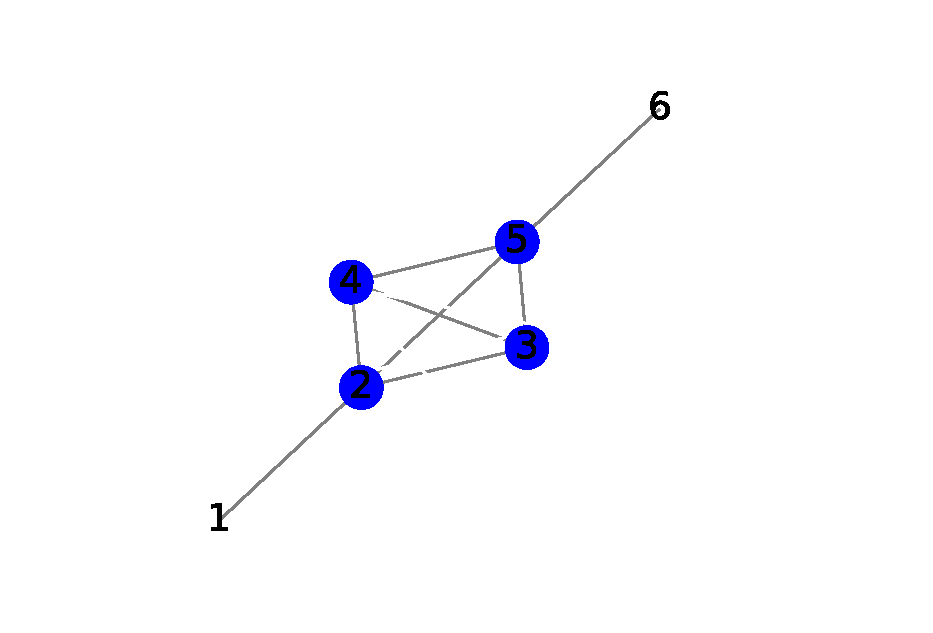
\includegraphics[scale=0.6]{grafo9}
  \caption{Proceso industrial de calidad}
  \label{imagen9}
\end{figure}

En la figura (\ref{imagen9}) el nodo 1 representa el inicio del proceso, los nodos intermedios (color azul) representan las actividades de revisión de calidad, las cuales se pueden llevar a cabo mas de una vez y el nodo 6 representa el fin del proceso.


%%%%%%%%%%%%%%%%%%%%%%%%%
%%%%%%%%%%%%%%%%%%%%%%%%%
%%%%%%%%%%%%%%%%%%%%%%%%%

\section*{Multigrafo dirigido acíclico }


Es un grafo $G = (N, A)$ que cumple:
\begin{itemize}
\item $G$ tiene al menos un par de nodos, tales que tienen mas de una arista de adyacencia.
\item Existe al menos un arco $(u, v) \ \epsilon \ A$ con dirección.
\item $G$ no tiene ciclos.
\end{itemize}


\textbf{Ejemplo:} (Red de vuelos en un aeropuerto). En la figura (\ref{imagen11}) se representa el número de viajes que puede existir entre un aeropuerto de una ciudad y otro de otra ciudad.

\begin{figure}[H]
  \centering
    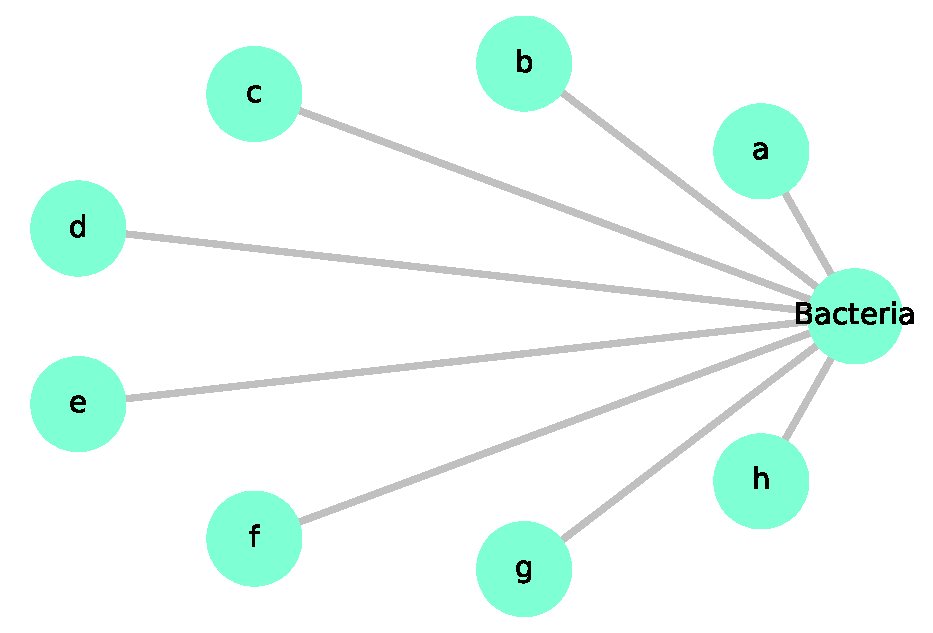
\includegraphics[scale=0.6]{grafo11}
  \caption{Red de vuelos}
  \label{imagen11}
\end{figure}

%%%%%%%%%%%%%%%%%%%%%%%%%
%%%%%%%%%%%%%%%%%%%%%%%%%
%%%%%%%%%%%%%%%%%%%%%%%%%



\section*{Multigrafo dirigido cíclico }

Es un grafo $G = (N, A)$ que cumple:
\begin{itemize}
\item $G$ tiene al menos un par de nodos, tales que tienen mas de una arista de adyacencia.
\item Existe al menos un arco $(u, v) \ \epsilon \ A$ con dirección.
\item $G$ al menos un ciclo.
\end{itemize}


\textbf{Ejemplo:} (Red de amistad). En la figura (\ref{imagen12}) se tiene un conjuto de personas que tienen agregado, son amigos, siguen, etc. a otra persona por algúna o algunas páginas de internet como Facebook, Instagram, Twiter, Hi-5, etc.

\begin{figure}[H]
  \centering
    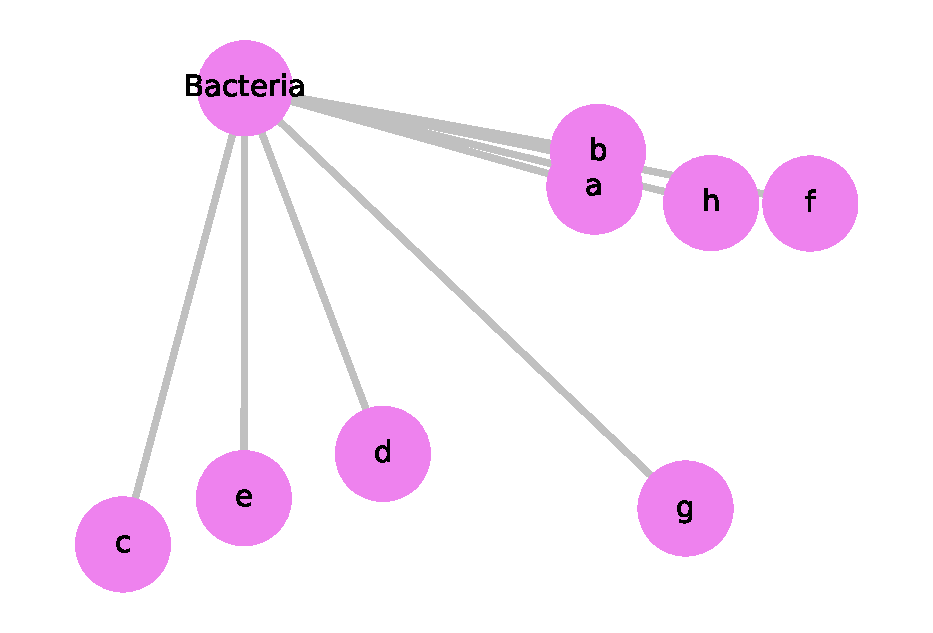
\includegraphics[scale=0.6]{grafo12}
  \caption{Redes sociales}
  \label{imagen12}
\end{figure}




%%%%%%%%%%%%%%%%%%%%%%%%%
%%%%%%%%%%%%%%%%%%%%%%%%%
%%%%%%%%%%%%%%%%%%%%%%%%%

\section*{Multigrafo dirigido reflexivo }


Es un grafo $G = (N, A)$ que cumple:
\begin{itemize}
\item $G$ tiene al menos un par de nodos, tales que tienen mas de una arista de adyacencia.
\item Existe al menos un arco $(u, v) \ \epsilon \ A$ con dirección.
\item $G$ tiene por lo menos un nodo $u$ tal que la relacion $(u, u) \ \epsilon \ A$.
\end{itemize}


\textbf{Ejemplo:} (Transmisión de enfermedades). En la figura (\ref{imagen12}) se representa la red social de un grupo de 6 personas los cuales pueden tener o desarrollar una cierta enfermedad, los arcos en la red representan la probabilidad de ser contagiado.


\begin{figure}[H]
  \centering
    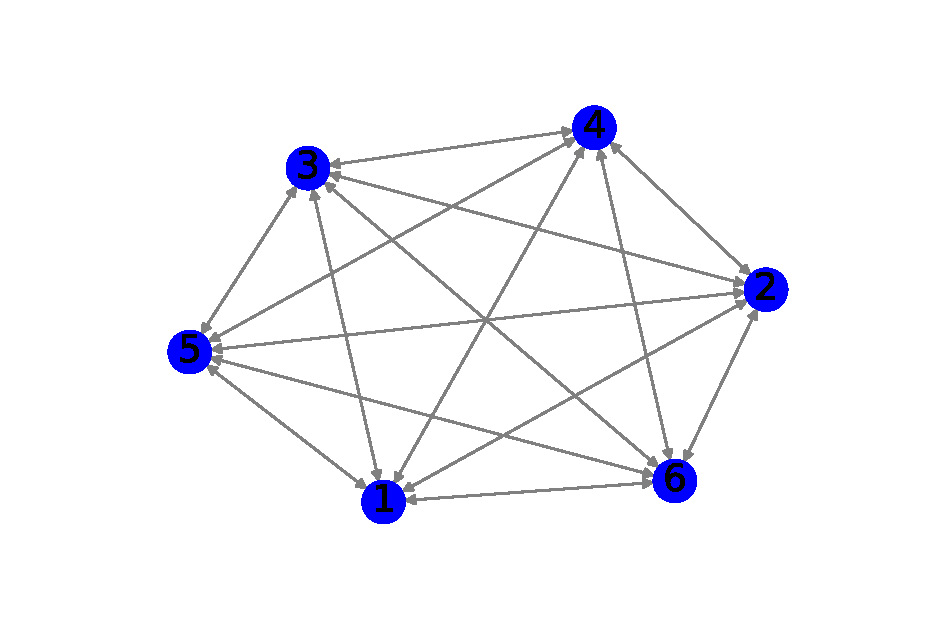
\includegraphics[scale=0.6]{grafo10}
  \caption{Transmisión de enfermedades}
  \label{imagen12}
\end{figure}

\bibliographystyle{unsrt}
\bibliography{bibliomi}
\nocite{*}

\end{document}